\begin{titlepage}

\centering \parindent=0pt
\newcommand{\HRule}{\rule{\textwidth}{1mm}}
\vspace*{\stretch{1}} \HRule\\[0.7cm]\Huge\bfseries
30010 - Programmeringsprojekt \\[0.7cm] % Kursusnummer og navn
Reflexball\\ % Titel
\HRule\\[2cm]  
\Large
Gruppe 3
\\
\large
Martin Boye Brunsgaard, s144012(1)	\\
Tore Gederaas Kanstad, s144021(2) \\
Peter Asbjørn Leer Bysted, s144045(3) \\
\begin{figure}[h]
\begin{center}
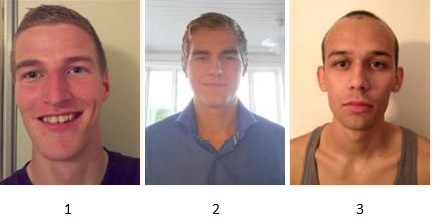
\includegraphics[scale=0.6]{img/faces.jpg}
\end{center}
\end{figure}

\vspace*{\stretch{1}} \normalsize

Alle medlemmer har været tilstede under øvelserne, og deltaget i udarbejdelse af journalerne. Ydermere har arbejdet været fordelt ligeligt over gruppemedlemerne, og løst i fællesskab. Rapporten er blevet udarbejdet og gennemlæst i kollektiv.
\vspace*{\stretch{1}}
\begin{flushleft}
Tecnical University of Denmark DTU\\ % Uddannelsesinstitusion
National Space Institute\\ 
30010 - Programming Project\\ % Kursusnummer og navn
25.06.2015 %Måned og år
\end{flushleft}
\end{titlepage}
\newpage
\renewcommand{\abstractname}{Abstract}
\begin{abstract}

This report is a mandatory part of the B.Sc. EE course 30010, Programming Project.\\ The report documents the entirety of this course, including the exercise journals and the final product, Reflexball, a program written in C and implemented on a microprocessor. \\ The first part of the course was learning how to use the ZDS II - Z8Encore! 4.9.3 tools, how to access the timers, the LED's, the buttons and how to use the PuTTY for displaying graphic. The code from these exercises were used to implement the HAL and some of the API for the project. The program was designed using a flow chart for the main function and a block diagram for the different program layers. The project was successfully implemented on a Z8 Encore Evaluation Board.
\end{abstract}
\renewcommand{\abstractname}{Resume}
\begin{abstract}
Denne rapport er en obligatorisk del af 30010, Programmeringsprojektet, som er en af de teknologiske linjefag på B.sc, EE. \\
Denne rapport dokumenterer helheden af dette kursus, inklusive journalerne og det endelige produkt, Reflexball, der er et program skrevet i C og implementeret på en mikroprocessor. I de første fire dage lærte forfatterne at bruge ZDS II - Z8Encore! 4.9.3 værktøjskassen, at konfigurere timerne, at vise strenge på LED'erne, at læse inputs fra knapperne og at bruge PuTTY til at vise grafik. Koden fra øvelserne blev brugt til at lave et HAL og en stor del af programmets API. Programmet blev designet ved hjælp af bla. flow charts og block diagrammer til at repræsentere programmets lag. Programmet blev med success implenteret på et Z8 Encore Evaluation Board.
\end{abstract}
\newpage
\tableofcontents


\newpage